% !TEX root = ../main.tex

\newlength\Radius
\setlength\Radius{2cm}

\section{Геометричні ймовірності. Аксіоми теорії ймовірностей.}
\subsection{Геометрична модель ймовірності}
\begin{example}
    Нехай точка кидається навмання на відрізок $\left[a; b\right]$. 
    Яка ймовірність її 
    потрапляння в $\left<\alpha; \beta\right> \subset  \left[a; b\right]$?
    Розглянемо подію $A = \left\{ 
        \text{точка потрапила в} \left<\alpha; \beta\right>
    \right\}$.
    \newline
    \hbox to \hsize{\hfil{
        \begin{tikzpicture}
            \draw [fill] (0, 0) circle [radius = 0.05];
            \node [below] at (0, 0) {$a$};
            \node [above] at (0, 0) { };
            \node [below] at (8, 0) {$b$};
            \draw [-{Straight Barb}] (6,0) to (2,0) {};
            \draw [-{Straight Barb}] (2,0) to (6,0) {};
            \node [below] at (2, 0) {$\alpha$};
            \node [below] at (6, 0) {$\beta$};
            \draw [fill] (8, 0) circle [radius = 0.05];
            \draw [thick] (0, 0) -- (8, 0);
        \end{tikzpicture}
    }\hfil}
    $P(A) = k\cdot l_{\left<\alpha; \beta\right>}\; \text{для деякого}\; k > 0$.
    З іншого боку, $P(\Omega) = 1 = k\cdot l_{\left[a; b\right]}$. Таким чином 
    $k = \frac{1}{l_{\left[a; b\right]}} = \frac{1}{b-a}$.
    Тому $P(A) = \frac{l_{\left<\alpha; \beta\right>}}{l_{\left[a; b\right]}}$.
\end{example}
Нехай простір елементарних подій інтерпретується як замкнена область в 
$ \mathbb{R} ^n$, а випадкові події --- її підмножини. В якості $\sigma$-алгебри 
подій $\mathcal{F}$ беремо підмножини, що мають міру $\mu$. Тоді в якості ймовірності 
деякої події $A$ беремо $P(A) = \frac{\mu(A)}{\mu(\Omega)}$. 
Наприклад, в $\mathbb{R}^1$ беремо міру <<довжина>>, в $\mathbb{R}^2$ --- <<площа>>, а в $\mathbb{R}^3$ --- <<об'єм>>.

Ймовірності, що знаходяться таким чином називаються \emph{геометричними}, а сама модель 
називається \emph{геометричною моделлю ймовірності}.
Геометрична модель може використовуватись, 
коли $\Omega$ має геометричну інтерпретацію як замкнена область в $\mathbb{R}^n$,
а елементарні події --- рівноможливі.

\begin{example}[задача Бюффона]\label{buffon}
    На площині накреслені паралельні прямі на відстані $2a$, на них кидається 
    голка довжиною $2l,\; l \leq a $. Яка ймовірність того, що голка перетне 
    яку-небудь пряму?
    \newline
    \hbox to \hsize{\hfil{
        \begin{tikzpicture}[scale = 0.5]
            \draw [thick] (0, 0) -- (8, 0);
            \draw [thick] (0, 2) -- (8, 2);
            \draw [thick] (0, 4) -- (8, 4);
            \draw [thick] (0, 6) -- (8, 6);
            \draw [{Straight Barb}-{Straight Barb}] (7.5,4) to (7.5,6);
            \node [right] at (7.5, 5) {$2a$}; 
        \end{tikzpicture}
        \begin{tikzpicture}[scale = 1]
            \draw (0, 0) -- (4, 0);
            \draw (0, 2) -- (4, 2);
            \draw [thick] (0.5, -0.5)-- (2.5, 1.5);
            \draw [{Straight Barb}-{Straight Barb}] (3.5,0) to (3.5,2);
            \draw [{Straight Barb}-{Straight Barb}] (1.5,0) to (1.5,0.5);
            \node [right] at (3.5, 1) {$2a$};
            \node [right] at (1.5, 0.25) {$ x $};
            \draw [-{Straight Barb}](2.5, 0) to [out = 90, in = 0](1.75, 0.75);
            \node [right] at (2.28, 0.53) {$ \varphi $};
        \end{tikzpicture}
    }\hfil}
    Достатньо розглядати лише дві прямі. $\Omega = \left\{(\varphi, x)\in 
    \mathbb{R}^2: \varphi \in \left[0; \pi\right], x \in \left[0; a\right] 
    \right\}$
    \newline
    При такій побудові простору елементарних подій подія $A = \left\{\text{голка 
    перетне пряму}\right\} =$
    \newline
    $\left\{(\varphi, x)\in 
    \Omega: x\leq l\sin\varphi\right\}$
    \newline
    \hbox to \hsize{\hfil{
        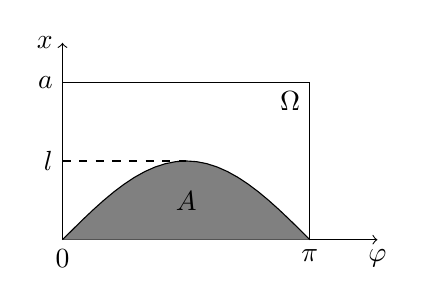
\begin{tikzpicture}
            \draw [<->] (4, 0) -- (0, 0) -- (0, 2.5);
            \node [left] at (0, 2.5) {$x$};
            \node [below] at (4, 0) {$\varphi$};
            \draw [domain=0:pi,fill=gray] plot (\x, {1*sin(\x r)});
            \node [below] at (0, 0) {$0$};
            \node [below] at (pi, 0) {$\pi$};
            \draw [dashed] (0,1) to (pi/2,1);
            \node [left] at (0, 1) {$l$};
            \draw (0,2) -- (pi, 2) -- (pi, 0);
            \node [left] at (0, 2) {$a$};
            \node [below left] at (pi, 2) {$\Omega$};
            \node [above] at (pi/2, 0.25) {$A$};
        \end{tikzpicture}
    }\hfil}
    $P(A) = \frac{S(A)}{S(\Omega)},\; S(\Omega) = \pi a,\;S(A) = \int\limits_0^\pi 
    l\sin\varphi\,\mathrm{d}x = l\left.(-\cos\varphi)\right|^\pi_0 = 2l$.
    Отже, $P(A) = \frac{2l}{\pi a}$.
    \newline
    Якщо провести $n$ кидань голки, у $m$ з яких голка потрапить на пряму, то за допомогою приблизної рівності $\frac{m}{n} 
    \approx \frac{2l}{\pi a}$ можна приблизно обчислити число $\pi$. 
    Наприклад, якщо взяти $n=5000, m=2532, l/a = 0.8$, то отримаємо $\pi \approx 3.1596$.
\end{example}
\begin{example}[парадокс Бертрана]
    Нехай в колі радіусом $R$ навмання обирається хорда. Яка ймовірність того, 
    що її довжина буде більшою за довжину сторони правильного трикутника, 
    вписаного в це коло?
    \newline
    Існують три способи розв'язання цієї задачі, причому кожен з них дає різний результат.
    
    \textbf{Спосіб 1.}
    З міркувань симетрії обирається якийсь фіксований діаметр кола і розглядається
    всі перпендикулярні до нього хорди. Серед них і обирається навмання довільна хорда.
    Очевидно, що кожна хорда у цьому випадку може бути однозначно визначена своєю серединою,
    тобто кожній хорді можна взаємно однозначно поставити у відповідність координату її середини,
    якщо за початок відліку взяти якийсь з кінців фіксованого діаметру.
    \newline
    \hbox to \hsize{\hfil{
        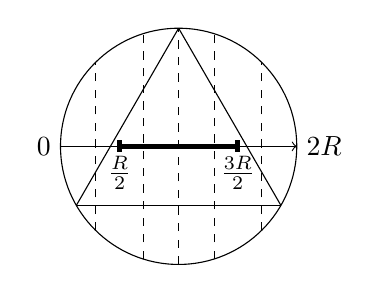
\begin{tikzpicture}[scale = 1.5]
            \draw (0, 0) circle [radius = 1]; 
            \draw (0, 1) -- (-0.86602540378, -0.5); 
            \draw (0, 1) -- (0.86602540378, -0.5);
            \draw (0.86602540378, -0.5) -- (-0.86602540378, -0.5);
            \draw [->] (-1,0) to (1, 0);
            \node [left] at (-1, 0) {$0$};
            \node [right] at (1, 0) {$2R$};
            \draw [dashed] (0, -1) to (0, 1);
            \draw [dashed] (-0.3, -0.954) to (-0.3, 0.954);
            \draw [dashed] (-0.7, -0.714) to (-0.7, 0.714);
            \draw [dashed] (0.3, -0.954) to (0.3, 0.954);
            \draw [dashed] (0.7, -0.714) to (0.7, 0.714);
            \draw [ultra thick] (-0.5, 0) -- (0.5, 0);
            \draw [ultra thick] (-0.5, 0.05) -- (-0.5, -0.05);
            \draw [ultra thick] (0.5, 0.05) -- (0.5, -0.05);
            \node [below] at (-0.5, 0) {$\frac{R}{2}$};
            \node [below] at (0.5, 0) {$\frac{3R}{2}$};
        \end{tikzpicture}
    }\hfil}
    Таким чином, множина всіх значень координати середини хорди $\Omega = \left[0; 2R\right]$. 
    Множина, що відповідає події --- це відрізок $A = \left[\frac{R}{2}; \frac{3R}{2}\right]$.
    В якості міри візьмемо довжину. Тоді $P(A) = \frac{l(A)}{l(\Omega)} = \frac{R}{2R}= \frac{1}{2}$.
    
    \textbf{Спосіб 2.}
    В цьому способі пропонується розглядати тільки хорди з одним закріпленим кінцем.
    Кожній хорді поставимо у відповідність ту частину дуги кола, яка потрапляє у кут $\varphi$,
    що утворює хорда з дотичною, проведеною через точку закріплення кінця всіх хорд.
    \newline
    \hbox to \hsize{\hfil{
        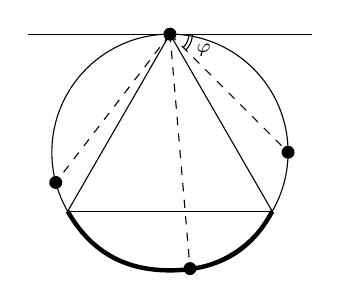
\begin{tikzpicture}[scale = 1.5]
            \draw (0, 0) circle [radius = 1];
            \draw (0, 1) -- (-0.86602540378, -0.5); 
            \draw (0, 1) -- (0.86602540378, -0.5);
            \draw (0.86602540378, -0.5) -- (-0.86602540378, -0.5);
            \draw (-1.2, 1) -- (1.2, 1);
            \draw [fill] (0, 1) circle [radius = 0.05];
            \draw [fill] (0.17, -0.985) circle [radius = 0.05];
            \draw [fill] (1, 0) circle [radius = 0.05];
            \draw [fill] (-0.967, -0.256) circle [radius = 0.05];
            \draw (0.16, 1) arc (0:-46:0.16);
            \draw (0.19, 1) arc (0:-46:0.19);
            %\node [above] at (0, 1);
            \draw [dashed] (0, 1) to (0.17, -0.985);
            \draw [dashed] (0, 1) to (1, 0);
            \draw [dashed] (0, 1) to (-0.967, -0.256);
            \node [below right] at (0.14, 1) {$_\varphi$};
            \draw [ultra thick](0.86602540378, -0.5) to [out = 242, in = 0](0, -1);
            \draw [ultra thick](0, -1) to [out = 180, in = 300](-0.86602540378, -0.5);
        \end{tikzpicture}
    }\hfil}
    Тоді множина $\Omega = \left[ 0; \pi\right]$, а $A = \left[ \frac{\pi}{3}; \frac{2\pi}{3}\right]$.
    Знову візьмемо за міру довжину і отримаємо $P(A) = \frac{\pi /3}{\pi} = \frac{1}{3}$.
    
    \textbf{Спосіб 3.}
    Розглядаються всі хорди кола. Кожній з них взаємно однозначно ставиться у відповідність точка її середини $(x,y)$,
    якщо за початок координат прийняти центр кола.
    \newline
    \hbox to \hsize{\hfil{
        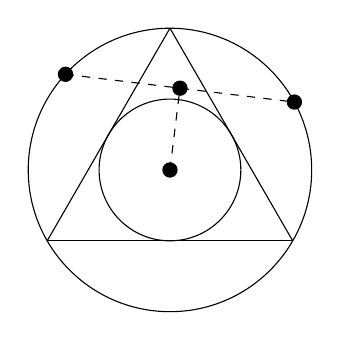
\begin{tikzpicture}[scale = 1.8]
            \draw (0, 0) circle [radius = 1];
            \draw (0, 0) circle [radius = 0.5];
            \draw (0, 0) [fill] circle [radius = 0.05];
            \draw (0, 1) -- (-0.86602540378, -0.5); 
            \draw (0, 1) -- (0.86602540378, -0.5);
            \draw (0.86602540378, -0.5) -- (-0.86602540378, -0.5);
            \draw (-0.737, 0.675) [fill] circle [radius = 0.05];
            \draw (0.878, 0.479) [fill] circle [radius = 0.05];
            \draw [dashed] (-0.737, 0.675) to (0.878, 0.479);
            \draw [dashed] (0, 0) to (0.0705, 0.577);
            \draw (0.0705, 0.577) [fill] circle [radius = 0.05];
        \end{tikzpicture}
    }\hfil}
    В такому випадку $\Omega = \left\{ (x,y)\in \mathbb{R}^2: x^2 + y^2 \leq R^2\right\}$,
    а $A = \left\{ (x,y)\in \Omega: x^2 + y^2 \leq \frac{R^2}{4}\right\}$.
    Тоді $P(A) = \frac{\pi R^2/4}{\pi R^2} = \frac{1}{4}$.

    Жозеф Бертран був противником геометричного означення ймовірності.
    Він казав, що воно не дає можливості однозначно обчислити ймовірність
    однієї і тієї ж випадкової події та використовував вищенаведений приклад
    для доведення своєї правоти. Дійсно, було отримано три різних відповіді при
    розв'язанні однієї задачі. Так в чому ж справа? Насправді, помилка полягає
    у різних трактуваннях поняття <<навмання обрана хорда>>.
    В кожному з трьох способів це трактування було різним, що й стало причиною різних відповідей.
\end{example}

\subsection{Аксіоми теорії ймовірностей}
\begin{enumerate}[label=\Roman*.]
    \item Побудова вимірного простору $\left\{ \Omega, \mathcal{F}\right\}$:
    \begin{enumerate}[label = \textbf{A\arabic*:}]
        \item Будь-якому стохастичному експерименту можна поставити у відповідність
        простір елементарних подій $\Omega$.
        \item $\left(\forall n \in \mathbb{N}: A_n \in \mathcal{F} \right) \Rightarrow \left( \bigcup\limits_{n=1}^{n (\infty)} A_n \in \mathcal{F}\right)$.
        \item $\left( A \in \mathcal{F}\right) \Rightarrow \left( \overline{A} \in \mathcal{F}\right)$.
        
        Дві останні аксіоми стосуються побудови алгебри чи $\sigma$-алгебри подій.
    \end{enumerate}
    \item Властивості ймовірності:
    \begin{enumerate}[label = \textbf{P\arabic*:}]
        \item $\forall A \in \mathcal{F}: P(A)\geq 0$.
        \item $P(\Omega) = 1$ --- аксіома нормування.
        \item $\forall A_1, A_2, ..., A_n, ... \in \mathcal{F},  A_i \cap A_j \text{ при } i \neq j: P\left(\bigcup\limits_{n=1}^{\infty} A_n\right) = \sum\limits_{n=1}^{\infty} P(A_n)$ ---
        аксіома зліченної адитивності.
        Іноді у випадках <<простої>> алгебри (а не $\sigma$-алгебри) достатньо
        аксіоми скінченної адитивності \textbf{P3$'$}: 
        $\forall A_1, A_2, ..., A_n \in \mathcal{F},  A_i \cap A_j \text{ при } i \neq j: P\left(\bigcup\limits_{k=1}^{n} A_k\right) = \sum\limits_{k=1}^{n} P(A_k)$.
    \end{enumerate}
\end{enumerate}
\begin{definition}
    Нормована міра $P$, що введена на вимірному просторі $\left\{ \Omega, \mathcal{F}\right\}$,
    називається \emph{ймовірністю}. Всі події беруться з $\sigma$-алгебри подій.
    Трійка $\left\{ \Omega, \mathcal{F}, P\right\}$ називається 
    \emph{ймовірнісний простором} стохастичного експерименту.
\end{definition}

Ця система аксіом несуперечна, бо існують стохастичні експерименти,
які задовольняють цим аксіомам, але неповна, бо в різних задачах
теорії ймовірностей розглядаються різні ймовірнісні простори.

\subsection{Властивості ймовірності, що випливають з аксіом}
\begin{enumerate}
    \item Якщо $A_1, A_2, ..., A_n, ... \in \mathcal{F}$ утворюють повну групу 
    подій, то $P\left(\bigcup\limits_{k=1}^\infty A_k\right) = 1$.
    \begin{proof}
        Випливає з аксіоми \textbf{P2}.
    \end{proof}
    \item $P(\overline{A}) = 1 - P(A)$.
    \begin{proof}
        $A \cup \overline{A} = \Omega \Rightarrow 1 \overset{P2}{=} P(\Omega) 
        = P(A \cup \overline{A}) \overset{P3'}{=} P(A) + P(\overline{A})$.
    \end{proof}
    \item $P(\varnothing) = 0$.
    \begin{proof}
        Наслідок з властивості 2 $(\varnothing = \overline{\Omega})$.
    \end{proof}
    \begin{remark}
        Якщо ймовірність події дорівнює нулю, то це не означає, що подія неможлива.
    \end{remark}
    \begin{example}
        СЕ --- кидання точки на відрізок $[a; b]$. A = \{\text{точка потрапила в 
        певну } $x \in [a; b]$\}. $A$ не є неможливою, проте $P(A) = 0$.
    \end{example}
    \item $A \subset B \Rightarrow P(A) \leq P(B)$.
    \begin{proof}
        $A \subset B \Rightarrow B = A \cup (B \backslash A) 
        \overset{P3'}{\Rightarrow} P(B) = P(A) + P(B \backslash A) 
        \overset{P1}{\geq} P(A)$.
    \end{proof}
    \item $\forall A \in \mathcal{F}: P(A) \leq 1$.
    \begin{proof}
        Наслідок з властивості 4, $A \subset \Omega$ та \textbf{P2}.
    \end{proof}
    \item $A \subset B: P(B \backslash A) = P(B) - P(A)$.
    \begin{proof}
        Наслідок з доведення властивості 4.
    \end{proof}
    \item $\forall A, B \in \mathcal{F}: P(A \cup B) = P(A) + P(B) - P(A \cap B)$.
    \begin{proof}
        $A \cup B = (A\backslash(A \cap B)) 
        \cup (A \cap B) 
        \cup (B\backslash(A \cap B))$ --- попарно несумісні події. 
        \newline
        З аксіоми \textbf{P3$'$}: $P(A \cup B) = P(A\backslash(A \cap B)) 
        + P(A \cap B) + P(B\backslash(A \cap B)) \overset{6}{=} P(A) - P(A \cap B) + P(A \cap B)
        + P(B) - P(A \cap B) = P(A) + P(B) - P(A \cap B)$.
    \end{proof}
    \item Узагальнення властивості 7 --- формула включення-виключення для ймовірностей: 
    
    \begin{math}
        \forall A_1, A_2, \dots, A_n \in \mathcal{F} 
    : P(\bigcup\limits_{i=1}^n A_i) = \sum\limits_{i=1}^n P(A_i) - \sum\limits_{i < j}^n P(A_i \cap A_j)
    + \sum\limits_{i < j < k}^n P(A_i \cap A_j \cap A_k) - ... + (-1)^{n-1}P\left(\bigcap\limits_{i=1}^n A_i\right)
    \end{math}.
    \nopagebreak
    \begin{exercise}
        Довести.
    \end{exercise}
\suspend{enumerate}
\begin{example}[задача про неуважну секретарку]
    Секретарка поклала $n$ листів в $n$ чистих конвертів, заклеїла ці конверти і тільки 
    після цього написала адреси. Яка ймовірність того, що хоча б один з листів дійде 
    за призначенням?
    \newline
    $A_i = \left\{i\text{-тий лист дійшов за призначенням}\right\}, i = 
    1,...,n. \;P(A_i) = \frac{1}{n} = \frac{(n-1)!}{n!}$.
    \newline
    $A = \left\{\text{хоча б один із листів дійшов за призначенням}\right\}, 
    A = \bigcup\limits_{i=1}^n A_i$.
    \newline
    $P(A_i \cap A_j) = \frac{(n-2)!}{n!} = \frac{1}{n(n-1)}, i \neq j$.
    \newline
    $P(A_i \cap A_j \cap A_k) = \frac{1}{n(n-1)(n-2)}, i \neq j \neq k$.
    \newline
    ...
    \newline
    $P(A_1 \cap ... \cap A_n) = \frac{1}{n!}$.
    \newline
    За формулою включення-виключення $P(A) = n\cdot \frac{1}{n} - C_n^2 \cdot \frac{1}{n(n-1)}- \dots + (-1)^{n-1}\frac{1}{n!}
    = 1 - \frac{1}{2!} + \frac{1}{3!} - \dots +(-1)^{n-1} \cdot \frac{1}{n!} \approx 
    1 - \frac{1}{e} \approx 0.63$.
\end{example}
\resume{enumerate}
    \item $\forall A_1, A_2, ..., A_n, ... \in \mathcal{F}: 
    P\left(\bigcup\limits_{k=1}^\infty A_k\right) \leq \sum\limits_{k=1}^\infty P(A_k)$
    \begin{proof}
        Введемо події $B_1 = A_1, B_2 = \overline{A_1} \cap A_2, 
        B_3 = \overline{A_1} \cap \overline{A_2} \cap A_3, ..., B_n = 
        \overline{A_1} \cap \overline{A_2} \cap ...$ 
        \newline
        $... \cap \overline{A_{n-1}} \cap A_n$. Ці події попарно несумісні, 
        $\bigcup\limits_{k=1}^\infty B_k = \bigcup\limits_{k=1}^\infty A_k,\;B_k \subset A_k $ для всіх $k \in \mathbb{N}$.
        \newline
        $P\left(\bigcup\limits_{k=1}^\infty A_k\right) = P\left(\bigcup\limits_{k=1}^\infty B_k\right) 
        \overset{P3}{=} \sum\limits_{k=1}^\infty P(B_k) \overset{4}{\leq} 
        \sum\limits_{k=1}^\infty P(A_k)$.
    \end{proof}
    \item $\forall A_1, A_2, ..., A_n, ... \in \mathcal{F}: P\left(\bigcap\limits_{k=1}^\infty
    A_k\right) = 1 - P\left(\overline{\bigcap\limits_{k=1}^\infty A_k}\right) = 1 - P\left(\bigcup\limits_{k=1}^\infty \overline{A_k}\right) \geq  
    1 - \sum\limits_{k=1}^\infty P(\overline{A_k})$.
\end{enumerate}

\subsection{Теореми неперервності ймовірності}
\begin{theorem}\label{th:1}
    Нехай є монотонно неспадна послідовність подій $A_1 \subset A_2 \subset ... \subset A_n ... \in \mathcal{F}$.
    Тоді $P\left(\bigcup\limits_{n=1}^{\infty} A_n\right) = \lim\limits_{n\rightarrow \infty} P(A_n)$.
\end{theorem}
\begin{proof}
    $\bigcup\limits_{n=1}^{\infty} A_n = A_1 \cup (A_2 \backslash A_1) \cup (A_3 \backslash A_2) \cup ... \cup (A_{n} \backslash A_{n-1}) \cup ...$ 

    \noindent З аксіоми \textbf{P3}: $P\left(\bigcup\limits_{n=1}^{\infty} A_n\right) = P(A_1) + \sum\limits_{n=2}^{\infty} P(A_{n} \backslash A_{n-1})$.

    \noindent $S_n = P(A_1) + \sum\limits_{k=2}^{n} P(A_{k} \backslash A_{k-1}) = P(A_1) + P(A_2) - P(A_1) + P(A_3) - P(A_2) + ... + P(A_n) - P(A_{n-1}) = P(A_n)$.
    Отже, $P\left(\bigcup\limits_{n=1}^{\infty} A_n\right) = \lim\limits_{n\rightarrow \infty} S_n = \lim\limits_{n\rightarrow \infty} P(A_n)$.
\end{proof}
\begin{theorem}\label{th:2}
    Нехай є монотонно спадна послідовність подій $A_1 \supset A_2 \supset ... \supset A_n ... \in \mathcal{F}$.
    Тоді $P\left(\bigcap\limits_{n=1}^{\infty} A_n\right) = \lim\limits_{n\rightarrow \infty} P(A_n)$.
\end{theorem}
\begin{proof}
    $P\left(\bigcap\limits_{n=1}^{\infty} A_n\right) = 1 - P\left(\bigcup\limits_{n=1}^{\infty} \overline{A_n}\right) \overset{\text{т. \refeq{th:1}}}{=} 1 -
    \lim\limits_{n\rightarrow \infty} P(\overline{A_n}) = \lim\limits_{n\rightarrow \infty} (1-P(\overline{A_n})) = \lim\limits_{n\rightarrow \infty} P(A_n)$.
\end{proof}
